\documentclass[accentcolor=tud9b, colorbacktitle, inverttitle]{tudbeamer}

\usepackage[utf8]{inputenc}
\usepackage[T1]{fontenc}
\usepackage[ngerman]{babel}
\usepackage{epstopdf}
\usepackage{graphicx}
\usepackage{xcolor}
\usepackage{tikz}
\usepackage{lipsum,multicol}
% \usepackage[backend=biber]{biblatex}
% \addbibresource{References_PSBeschl_2018.bib}

% style=alphabetic, 
\usepackage{tikz}						% graphics creation environment frontend
\usepackage{tikz-cd}
\usepackage{import}
\usepackage{multicol}
\usepackage{subfig}
% 
\usepackage{pgfplots}					% graph plotting for pgf/tikz
\pgfplotsset{compat=1.12, grid style={gray,dotted}}

%\usetikzlibrary{external} %% comment out to stop externalization of tikz pictures
%\tikzexternalize[optimize=false, prefix=tikz-external/] % path to store the externalized stuff in
%\tikzset{external/system call={lualatex \tikzexternalcheckshellescape -halt-on-error-interaction=batchmode -jobname "\image" "\texsource"}, force remake = false}
%% \tikzset{external/force remake = false}
%\tikzexternalize

\graphicspath{{graph/}}

\author{Julian Buschbaum, Benjamin Northe, Rainer Stellnberger}
\institute{Institut TEMF}
\logo[1.5]{\includegraphics{temf}}
\date{\today}
\title{Parameteranalyse von kurzgeschlossenen Ringkernen mittels Impedanzmessung}

\begin{document}

\begin{titleframe}
\vspace{-1em}
	\begin{figure}[h]
		\centering
		\includegraphics[width=0.72\textwidth]{Kavitaet}
	\end{figure}
\end{titleframe}





\begin{frame}\frametitle{Inhalt}
	\begin{itemize}
		\item Aufgabenstellung
		\item Der Messaufbau
		\item Durchgef\"uhrte Simulationen
		\item Modifikation der Testbox
	\end{itemize}
\end{frame}


\begin{frame}\frametitle{Aufgabenstellung}
\begin{multicols}{2}
\vspace{-2em}
	\begin{figure}[h]
		\centering
		\includegraphics[width=0.5\textwidth]{Kavitaet}
	\end{figure}
	\vfill\null
	\columnbreak
	\begin{itemize}
		\item MA(Magnetic Alloy)-Ringkerne zur Stimmung der Kavit\"at
		\item Im passiven Betrieb der Kavit\"at m\"oglichst wenig Einfluss auf den Strahl gewünscht (Impendanz)
		\item Theorie: Kurzschlussschaltung um die Ringkerne soll deren Einfluss auf die Impedanz reduzieren
	\end{itemize}
\end{multicols}
\end{frame}


\begin{frame}\frametitle{Der Messaufbau}
\vspace{-2em}
	\begin{figure}[h]
		\centering
		\includegraphics[width=0.72\textwidth]{opentest}
	\end{figure}
\end{frame}




\begin{frame}\frametitle{Bisherige Messungen}
\begin{multicols}{2}
	\vspace{-2em}
	\begin{figure}[h]
		\centering
		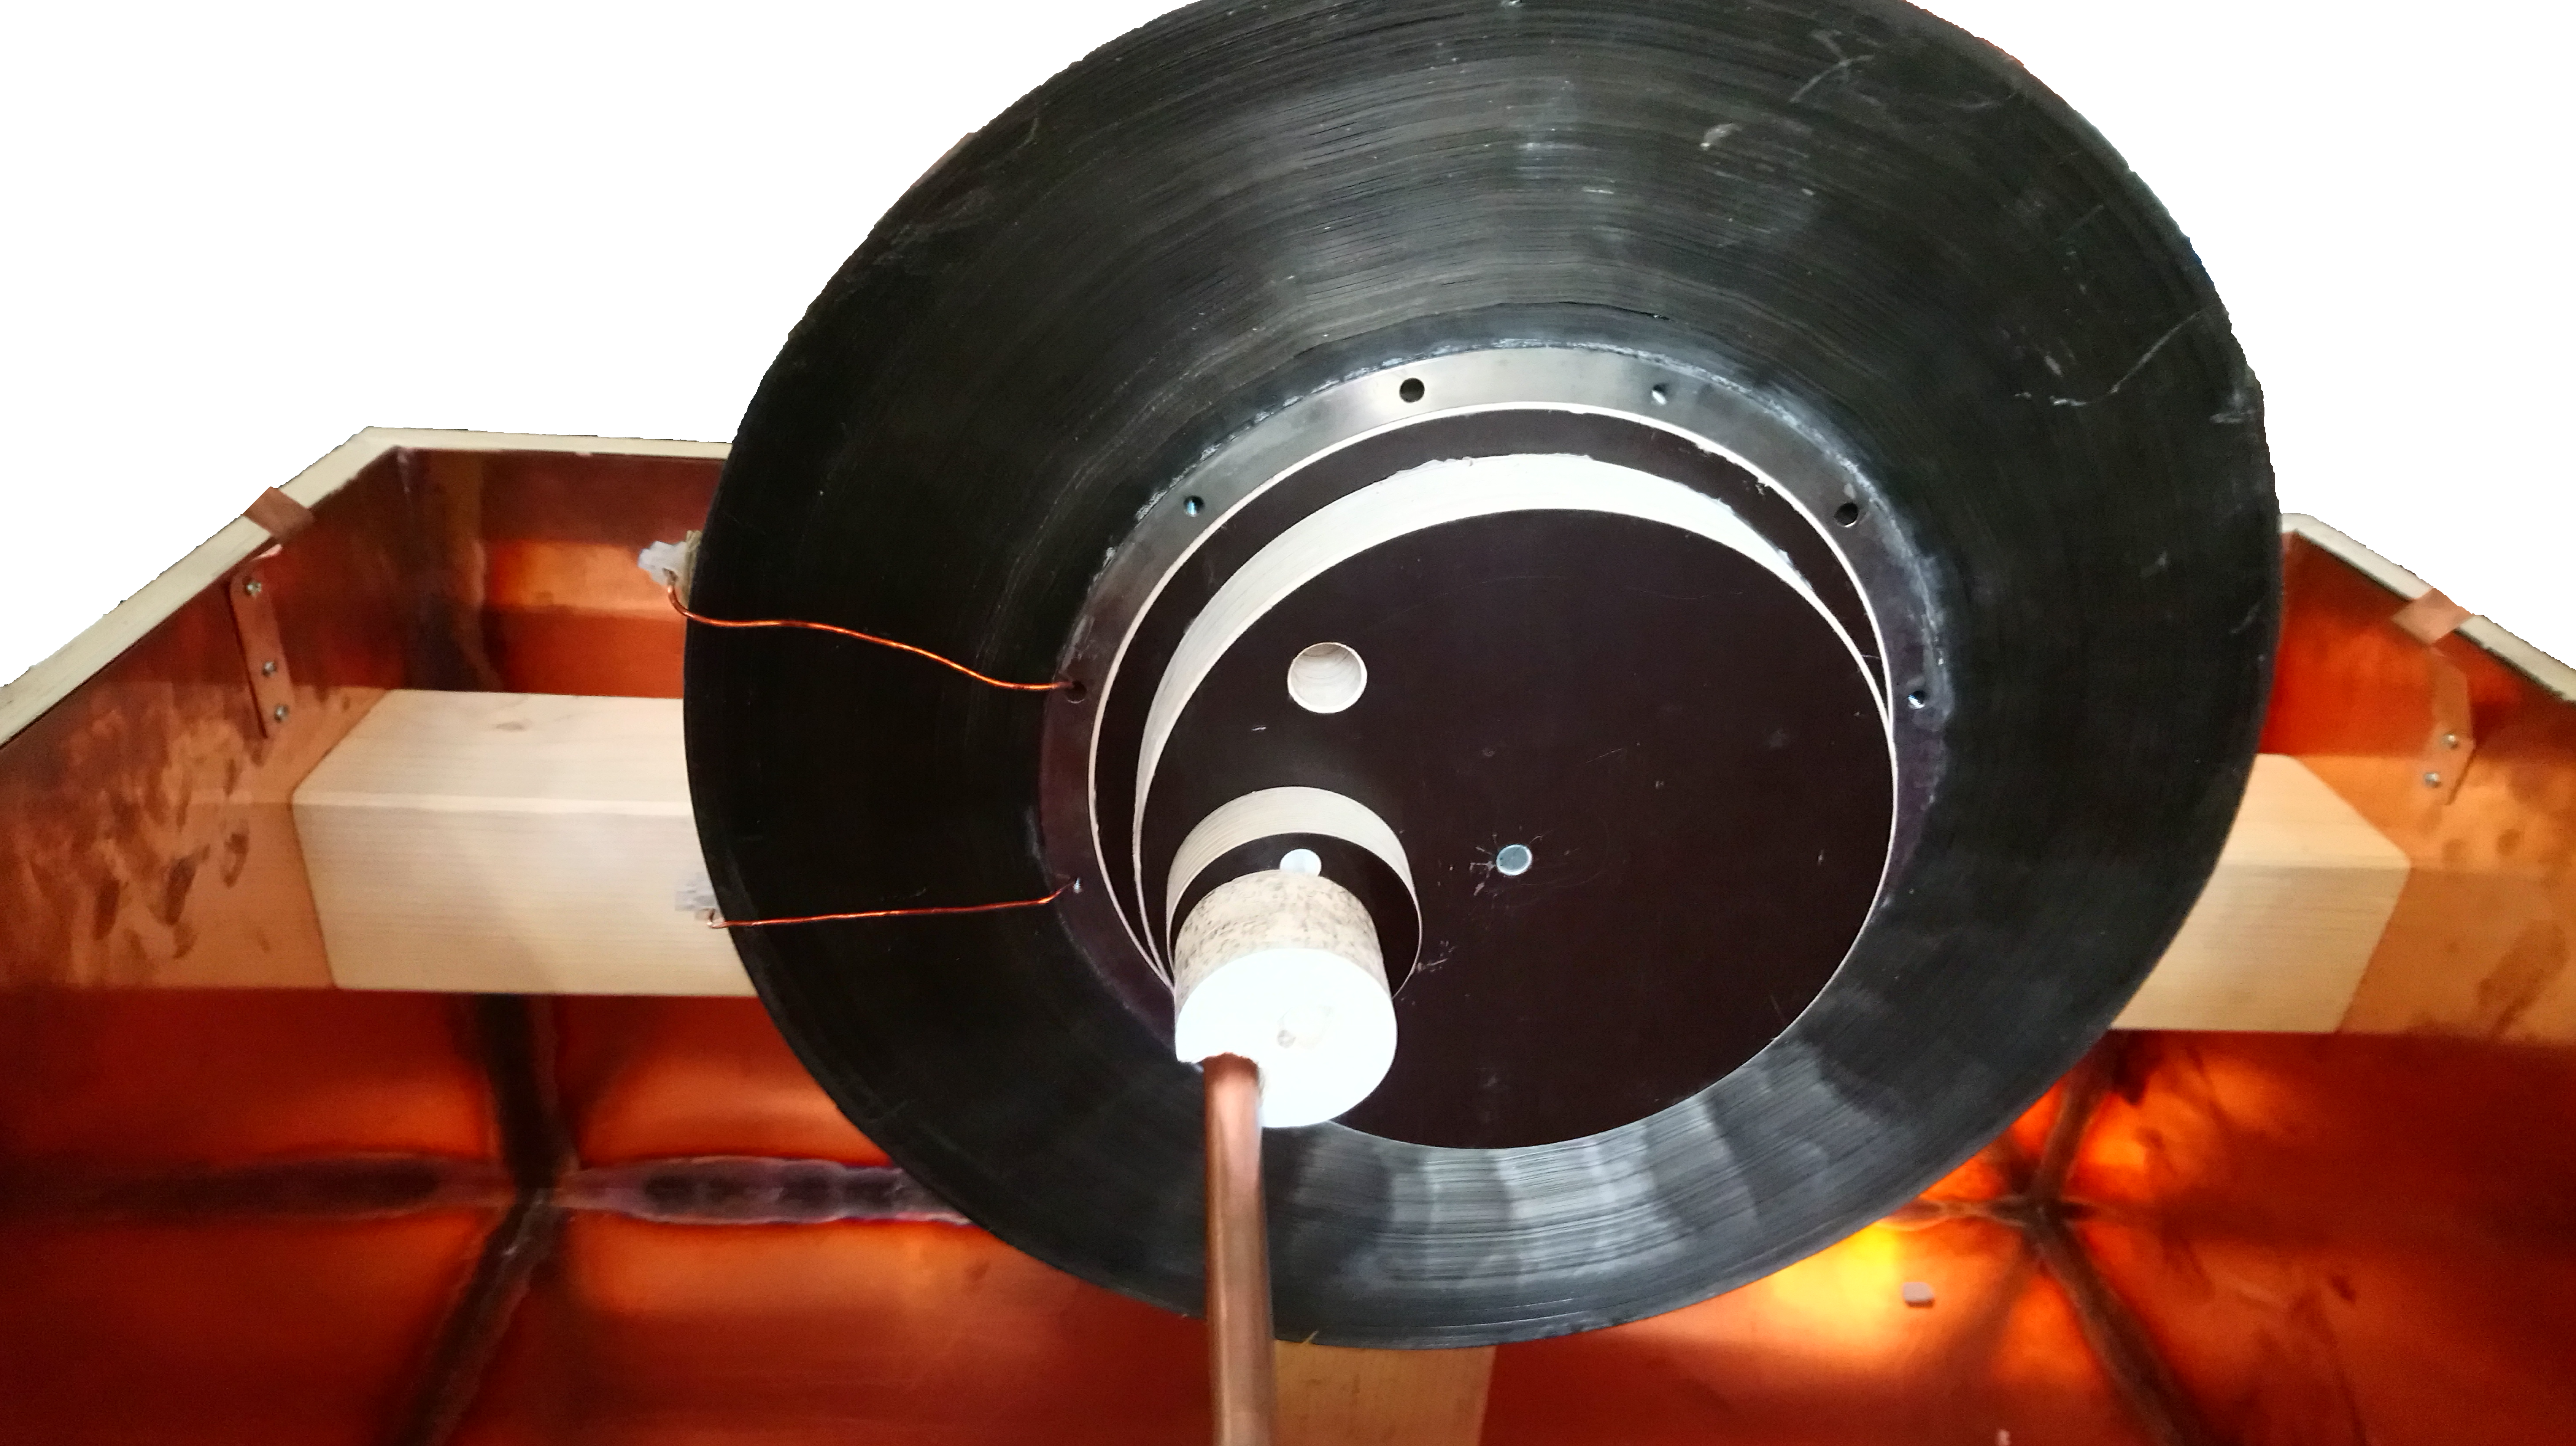
\includegraphics[width=0.5\textwidth]{test_ks_adapted_v2}
	\end{figure}
	\vfill\null
	\columnbreak
	\begin{itemize}
		\item Fixierung der Kurzschl\"usse schwierig
		\item Messung dadurch nur bedingt reproduzierbar
	\end{itemize}

\end{multicols}
\end{frame}




\begin{frame}\frametitle{Simulationen}
Mithilfe von CST wurden mehrere Faktoren f\"ur die Kurzschl\"usse durchsimuliert:
\begin{itemize}
	\item Anzahl der Kurzschl\"usse
	\item Positionen der Kurzschl\"usse
	\item Formen der Kurzschl\"usse
	\item Verschiedene Abst\"ande der Kurzschlusswicklung zum Ringkern
	\item Feldimpedanz mit einer unterbrochenen Schiene (wenn sich diese im Leerlauf befindet)
\end{itemize}
\end{frame}




\begin{frame}\frametitle{Feldimpedanz f\"ur verschiedene Anzahlen an Kurzschl\"ussen}
\vspace{-2em}
\begin{figure}[h]
	\subfloat[]{\includegraphics[height = 0.3\textwidth]{1ksTorus}} \hspace{1em}
	\subfloat[]{\includegraphics[height = 0.3\textwidth]{4ksTorus}}\hspace{1em}
	\subfloat[]{\includegraphics[height = 0.3\textwidth]{24ksTorus}}
\end{figure}
\end{frame}




\begin{frame}\frametitle{Feldimpedanz f\"ur verschiedene Anzahlen an Kurzschl\"ussen}
\vspace{-2em}
\begin{figure}[h]
	\centering
	\begin{tikzpicture}
		\begin{axis}[width=0.85\textwidth, height = 0.58\textwidth, xmin = 0.1, xmax = 50, xlabel=Frequenz in MHz, ylabel=Realteil der Impedanz der Box in Ohm, xticklabel style={/pgf/number format/fixed,/pgf/number format/precision=5}, every axis plot/.append style={thick},every axis legend/.append style={at={(0,1)},anchor=north west}, grid=both, cycle list name=color list]
			\addplot table[x index=0,y index=1,mark=none] {graph/plotData/Box.txt};
			\addplot table[x index=0,y index=1,mark=none] {graph/plotData/Rk.txt};
			\addplot table[x index=0,y index=1,mark=none] {graph/plotData/Rk1Ks0.txt};
			\addplot table[x index=0,y index=1,mark=none] {graph/plotData/Rk4Ks90.txt};
			\addplot table[x index=0,y index=1,mark=none] {graph/plotData/Rk24Ks15.txt};
			\legend{\small leere Box,\small Box mit Ringkern,\small 1 Kurzschluss,\small 4 Kurzschl\"usse (90 Grad versetzt),\small  24 Kurzschl\"usse}
		\end{axis}
	\end{tikzpicture}
\end{figure}
\end{frame}




\begin{frame}\frametitle{Feldimpedanz f\"ur verschiedene Positionen der Kurzschl\"usse}
\vspace{-2em}
\begin{figure}[h]
	\subfloat[]{\includegraphics[height = 0.4\textwidth]{4ksTorus}} \hspace{1em}
	\subfloat[]{\includegraphics[height = 0.4\textwidth]{4ksTorus30Grad}}
\end{figure}
\end{frame}




\begin{frame}\frametitle{Feldimpedanz f\"ur verschiedene Positionen der Kurzschl\"usse}
\vspace{-2em}
\begin{figure}[h]
	\centering
	\begin{tikzpicture}
		\begin{axis}[width=0.85\textwidth, height = 0.5\textwidth, xmin = 0.1, xmax = 50, xlabel=Frequenz in MHz, ylabel=Realteil der Impedanz der Box in Ohm, xticklabel style={/pgf/number format/fixed,/pgf/number format/precision=5}, every axis plot/.append style={thick},every axis legend/.append style={at={(0,1)},anchor=north west}, grid=both, cycle list name=color list]
			\addplot table[x index=0,y index=1,mark=none] {graph/plotData/Box.txt};
			\addplot table[x index=0,y index=1,mark=none] {graph/plotData/Rk.txt};
			\addplot table[x index=0,y index=1,mark=none] {graph/plotData/Rk4Ks30.txt};
			\addplot table[x index=0,y index=1,mark=none] {graph/plotData/Rk4Ks90.txt};
			\legend{\small leere Box, \small Box mit Ringkern, \small 4 Kurzschl\"usse (30 Grad versetzt), \small 4 Kurzschl\"usse (90 Grad versetzt)}
		\end{axis}
	\end{tikzpicture}
\end{figure}
\end{frame}




\begin{frame}\frametitle{Feldimpedanz f\"ur verschiedene Formen der Kurzschl\"usse (jeweils 1 KS)}
\vspace{-2em}
\begin{figure}[h]
	\subfloat[]{\includegraphics[height = 0.3\textwidth]{1ksTorus}} \hspace{1em}
	\subfloat[]{\includegraphics[height = 0.3\textwidth]{1ksSchiene}}\hspace{1em}
	\subfloat[]{\includegraphics[height = 0.3\textwidth]{1ksSchieneSchmal}}
\end{figure}
\end{frame}




\begin{frame}\frametitle{Feldimpedanz f\"ur verschiedene Formen der Kurzschl\"usse (jeweils 1 KS)}
\vspace{-2em}
\begin{figure}[h]
	\centering
	\begin{tikzpicture}
		\begin{axis}[width=0.85\textwidth, height = 0.5\textwidth, xmin = 0.1, xmax = 50, xlabel=Frequenz in MHz, ylabel=Realteil der Impedanz der Box in Ohm, xticklabel style={/pgf/number format/fixed,/pgf/number format/precision=5}, every axis plot/.append style={thick},every axis legend/.append style={at={(0,1)},anchor=north west}, grid=both, cycle list name=color list]
			\addplot table[x index=0,y index=1,mark=none] {graph/plotData/Box.txt};
			\addplot table[x index=0,y index=1,mark=none] {graph/plotData/Rk.txt};
			\addplot table[x index=0,y index=1,mark=none] {graph/plotData/Rk1Ks0.txt};
			\addplot table[x index=0,y index=1,mark=none] {graph/plotData/Kupferschiene.txt};
			\addplot table[x index=0,y index=1,mark=none] {graph/plotData/KupferschieneSchmal.txt};
			\legend{\small leere Box, \small Box mit Ringkern, \small 1 Kurzschluss(Torus), \small 1 Kupferschiene, \small 1 Kupferschiene (schmal)}
		\end{axis}
	\end{tikzpicture}
\end{figure} 
\end{frame}




\begin{frame}\frametitle{Feldimpedanz f\"ur verschiedene Formen der Kurzschl\"usse (jeweils 4 KS)}
\vspace{-2em}
\begin{figure}[h]
	\centering
	\begin{tikzpicture}
		\begin{axis}[width=0.85\textwidth, height = 0.5\textwidth, xmin = 0.1, xmax = 50, xlabel=Frequenz in MHz, ylabel=Realteil der Impedanz der Box in Ohm, xticklabel style={/pgf/number format/fixed,/pgf/number format/precision=5}, every axis plot/.append style={thick},every axis legend/.append style={at={(0,1)},anchor=north west}, grid=both, cycle list name=color list]
			\addplot table[x index=0,y index=1,mark=none] {graph/plotData/Box.txt};
			\addplot table[x index=0,y index=1,mark=none] {graph/plotData/Rk.txt};
			\addplot table[x index=0,y index=1,mark=none] {graph/plotData/Rk4Ks90.txt};
			\addplot table[x index=0,y index=1,mark=none] {graph/plotData/Kupferschiene4x.txt};
			\legend{\small leere Box, \small Box mit Ringkern, \small 4 Kurzschl\"usse(Torus), \small 4 Kupferschienen}
		\end{axis}
	\end{tikzpicture}
\end{figure}
\end{frame}




\begin{frame}\frametitle{Feldimpedanz f\"ur verschiedene Abst\"ande der Kurzschlusswicklung zum Ringkern}
\vspace{-2em}
\begin{figure}[h]
	\centering
	\includegraphics[width=0.45\textwidth]{1ksSchieneWeit}
\end{figure}
\end{frame}




\begin{frame}\frametitle{Feldimpedanz f\"ur verschiedene Abst\"ande der Kurzschlusswicklung zum Ringkern}
\vspace{-2em}
\begin{figure}[h]
	\centering
	\begin{tikzpicture}
		\begin{axis}[width=0.85\textwidth, height = 0.5\textwidth, xmin = 0.1, xmax = 50, xlabel=Frequenz in MHz, ylabel=Realteil der Impedanz der Box in Ohm, xticklabel style={/pgf/number format/fixed,/pgf/number format/precision=5}, every axis plot/.append style={thick},every axis legend/.append style={at={(0,1)},anchor=north west}, grid=both, cycle list name=color list]
			\addplot table[x index=0,y index=1,mark=none] {graph/plotData/Box.txt};
			\addplot table[x index=0,y index=1,mark=none] {graph/plotData/Rk.txt};
			\addplot table[x index=0,y index=1,mark=none] {graph/plotData/Kupferschiene.txt};
			\addplot table[x index=0,y index=1,mark=none] {graph/plotData/KupferschieneAbstandsvariation.txt};
			\addplot table[x index=0,y index=1,mark=none] {graph/plotData/KupferschieneEngRK.txt};
			\legend{\small leere Box,\small Box mit Ringkern,\small 1 Kupferschiene,\small 1 Kupferschiene (weiter Abstand),\small 1 Kupferschiene (eng am Ringkern)}
		\end{axis}
	\end{tikzpicture}
\end{figure}
\end{frame}




\begin{frame}\frametitle{Feldimpedanz mit einer unterbrochenen Schiene (wenn sich diese im Leerlauf befindet)}
\vspace{-2em}
\begin{figure}[h]
	\centering
	\includegraphics[width=0.35\textwidth]{1ksSchieneOffen}
\end{figure}
\end{frame}




\begin{frame}\frametitle{Feldimpedanz mit einer unterbrochenen Schiene (wenn sich diese im Leerlauf befindet)}
\vspace{-2em}
\begin{figure}[h]
	\centering
	\begin{tikzpicture}
		\begin{axis}[width=0.85\textwidth, height = 0.5\textwidth, xmin = 0.1, xmax = 50, xlabel=Frequenz in MHz, ylabel=Realteil der Impedanz der Box in Ohm, xticklabel style={/pgf/number format/fixed,/pgf/number format/precision=5}, every axis plot/.append style={thick},every axis legend/.append style={at={(1,0)},anchor=south east}, grid=both, cycle list name=color list]
			\addplot table[x index=0,y index=1,mark=none] {graph/plotData/Rk.txt};
			\addplot table[x index=0,y index=1,mark=none] {graph/plotData/KupferschieneOffen.txt};
			\legend{\small Box mit Ringkern, \small Box mit einer offenen Kupferschiene}
		\end{axis}
	\end{tikzpicture}
\end{figure}
\end{frame}




\begin{frame}\frametitle{Feldimpedanz mit vier unterbrochenen Schienen (wenn sich diese im Leerlauf befinden)}
\vspace{-2em}
\begin{figure}[h]
	\centering
	\begin{tikzpicture}
		\begin{axis}[width=0.85\textwidth, height = 0.5\textwidth, xmin = 0.1, xmax = 50, xlabel=Frequenz in MHz, ylabel=Realteil der Impedanz der Box in Ohm, xticklabel style={/pgf/number format/fixed,/pgf/number format/precision=5}, every axis plot/.append style={thick},every axis legend/.append style={at={(1,0)},anchor=south east}, grid=both, cycle list name=color list]
			\addplot table[x index=0,y index=1,mark=none] {graph/plotData/Rk.txt};
			\addplot table[x index=0,y index=1,mark=none] {graph/plotData/KupferschieneOffen4x.txt};
			\legend{\small Box mit Ringkern, \small Box mit vier offenen Kupferschienen}
		\end{axis}
	\end{tikzpicture}
\end{figure}
\end{frame}




\begin{frame}\frametitle{Feldimpedanz mit vier unterbrochenen Schienen (wenn sich diese im Leerlauf befinden)}
\vspace{-2em}
\begin{figure}[h]
	\centering
	\begin{tikzpicture}
		\begin{axis}[ymode=log, width=0.85\textwidth, height = 0.5\textwidth, xmin = 0.1, xmax = 100, xlabel=Frequenz in MHz, ylabel=Realteil der Impedanz der Box in Ohm, xticklabel style={/pgf/number format/fixed,/pgf/number format/precision=5}, every axis plot/.append style={thick},every axis legend/.append style={at={(1,0)},anchor=south east}, grid=both, cycle list name=color list]
			\addplot table[x index=0,y index=1,mark=none] {graph/plotData/Rk.txt};
			\addplot table[x index=0,y index=1,mark=none] {graph/plotData/KupferschieneOffen4x.txt};
			\legend{\small Box mit Ringkern, \small Box mit vier offenen Kupferschienen}
		\end{axis}
	\end{tikzpicture}
\end{figure}
\end{frame}


\begin{frame}\frametitle{Modifikation der Testbox}
\begin{multicols}{2}
\vspace{-2em}
	\begin{figure}[h]
		\centering
		\includegraphics[width=0.45\textwidth]{halterung}
	\end{figure}
	\vfill\null
	\columnbreak
	\begin{itemize}
		\item Montage der Kurzschl\"usse an verschiedenen Positionen 
		\item Vergleichbarkeit, durch feste Positionen
		\item Variable Anzahl von Kurzschl\"ussen m\"oglich
	\end{itemize}

\end{multicols}
\end{frame}


\begin{frame}\frametitle{Ausblick}
Was steht jetzt noch an:
        \begin{itemize}
            \item Montage der neuen Halterung
            \item Messung der simulierten Kurzschlussanordnungen
            \item Vergleich von Simulation und Messung
            \item Bewertung der Einflussfaktoren
            \item Ausarbeiten einer favorisierten Umsetzung der Kurzschlussanordnung
            \item Übertragen der Teststandmessung auf die Breitbandkavität
            
        \end{itemize}

\end{frame}

% \begin{frame}\frametitle{Quellen}
% % 	\bibliographystyle{plain}
% 	\bibliography{References_PSBeschl_2018.bib} 
% \end{frame}



\end{document}
